\documentclass[tikz, preview]{standalone}

\usepackage{amsfonts, amsthm, amssymb, amsmath, stmaryrd, etoolbox}
\usepackage{tikz}
\usetikzlibrary{matrix,arrows}
\tikzset{zxgreen/.style={shape=circle,thick,draw,fill=green}}
\tikzset{zxred/.style={shape=circle,draw,thick,fill=red}}
\tikzset{zxyellow/.style={shape=rectangle,draw,thick,fill=yellow}}
\tikzset{zxdiamond/.style={shape=diamond,fill=black,inner sep=2.75}}
\tikzset{zxopen/.style={shape=circle,draw,thick,inner sep=2pt}}
\tikzset{->-/.style={decoration={markings,mark=at position .5 with {\arrow{>}}},postaction={decorate}}}
\tikzset{->-pos/.style={decoration={markings,mark=at position #1 with {\arrow{>}}},postaction={decorate}}}


\begin{document}

\[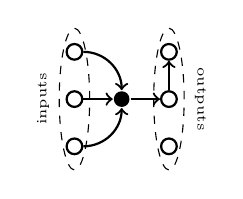
\begin{tikzpicture}
\begin{scope}
\node [circle,draw,inner sep=2pt,thick] (1) at (-.2,0.6) {};
\node [circle,draw,inner sep=2pt,thick] (2) at (-.2,0) {};
\node [circle,draw,inner sep=2pt,thick] (3) at (-.2,-0.6) {};
\node [circle,fill,inner sep=2pt,thick] (4) at (-.8,0) {};
\node [circle,draw,inner sep=2pt,thick] (5) at (-1.4,0.6) {};
\node [circle,draw,inner sep=2pt,thick] (6) at (-1.4,0) {};
\node [circle,draw,inner sep=2pt,thick] (7) at (-1.4,-0.6) {};
%
\draw [thick,->] (7) edge[out=0,in=-90] (4);
\draw [thick,->] (6) edge (4);
\draw [thick,->] (5) edge[out=0,in=90] (4);
\draw [thick,->] (4) edge (2);
\draw [thick,->] (2) edge (1);
%
\draw [dashed] (-1.4,0) ellipse (0.55em and 0.9cm);
\node [rotate=90] at (-1.8,0) {\tiny inputs};
\draw [dashed] (-0.2,0) ellipse (0.55em and 0.9cm);
\node [rotate=-90] at (0.2,0) {\tiny outputs};
\end{scope}
\end{tikzpicture}
\]

\end{document}
